\newpage % Rozdziały zaczynamy od nowej strony.
\section{Przegląd literatury}
Problem rozpoznawania dyscypliny sportu jest pod-problemem rozpoznawania aktywności. Rozpoznawanie aktywności można podzielić na trzy poziomy \cite{Wu2021}:
\begin{itemize} 
\item Aktywności indywidualne -  skupiające się na czynnościach wykonywanych przez jedną osobę. W takim kontekście, szczegółowe cechy sylwetki oraz dynamika ruchu ciała dostarczają wystarczających danych do precyzyjnej klasyfikacji.
\item Aktywności grupowe - dotyczą akcji, w których możemy rozróżnić indywidualne sylwetki, ale ich czynności nie są do końca jednoznaczne. W takim przypadku musimy uwzględnić interakcje pomiędzy uczestnikami oraz spojrzeć na całość sytuacji, nie skupiając się tylko na indywidualnych ruchach
\item Aktywności tłumu - brak możliwości analizowania indywidualnych osób,  należy patrzyć na akcje jako całość
\end{itemize}
Klasyfikacja dyscyplin sportowych jest kombinacją klasyfikacji aktywności indywidualnych oraz grupowych. 

Problem rozpoznawania aktywności jest badany już od długiego czasu, jednak w dużej mierze opiera się on na badaniu aktywności indywidualnych. Skupia się on na wykorzystywaniu ręcznie zaprojektowanych cech. Rozpowszechnienie się uczenia głębokiego otworzyło nowe możliwości w tej dziedzinie, a modele oparte na tej metodzie osiągają dotychczas najlepsze skuteczności. W tym rozdziale omówione zostaną prace istotne lub podobne do tej.  

\subsection{Modele hierarchiczne uczenia głębokiego}
Modele hierarchiczne opierają się na założeniu, że aby zrozumieć aktywność grupową, konieczne jest indywidualne analizowanie akcji każdej z poszczególnych osób. Wynikowa aktywność jest efektem klasyfikacji wartości funkcji agregującej cechy poszczególnych osób. To podejście wymaga intensywnego wstępnego przetworzenia nagrania, które obejmuje identyfikację poszczególnych osób, śledzenie ich detekcji w sekwencji, a także ekstrakcję unikalnych cech tych osób, takich jak cechy szkieletowe czy cechy RGB.
\subsubsection{Hierarchiczne modele splotowe}
Fabio Zappardino et al.\cite{Szkielety} w swojej pracy proponuje podejście oparte na cechach sylwetkowych poszczególnych osób oraz kombinacji ich przy pomocy sieci splotowych CNN. Zaproponowana w pracy architektura składa się z trzech gałęzi o identycznej strukturze, ale oddzielnych wagach, gdzie każda z gałęzi modelu przyjmuje na wejściu ręcznie wyselekcjonowane cechy, oparte na danych szkieletowych wyekstrahowanych przy pomocy modelu OpenPose \cite{openpose}. Przyjmowane cechy to: 
\begin{itemize}
    \item Ruch wyrażony poprzez skonkatenowane wektory przedstawiające pozy w kolejnych klatkach jednej osoby 
    \item Ruch wyrażony poprzez wyliczenie przesunięcia każdego z wyznaczonych stawów
    \item Zależność do pozostałych członków grupy, poprzez wyliczenie różnicy stawów między analizowanym uczestnikiem, a wybranym dla akcji uczestnikiem centralnym
\end{itemize}
Wyjścia z sieci splotowych są konkatenowane oraz trafiają do kolejnej warstwy splotowej, której odpowiedzialnością jest zakodowanie ruchu poszczególnych osób.

Tego typu przetwarzanie zostaje nałożone na każdą z osób biorącą udział w aktywności oraz zebrane do wspólnej macierzy, na którą nałożona zostaje transformacja MaxPooling'u po osobach. Tak przetworzona macierz trafia do modelu klasyfikującego. Architektura całego systemu została przedstawiona na rysunku \ref{fig:szkielety-arch}.
\begin{figure}[!h]
    \centering 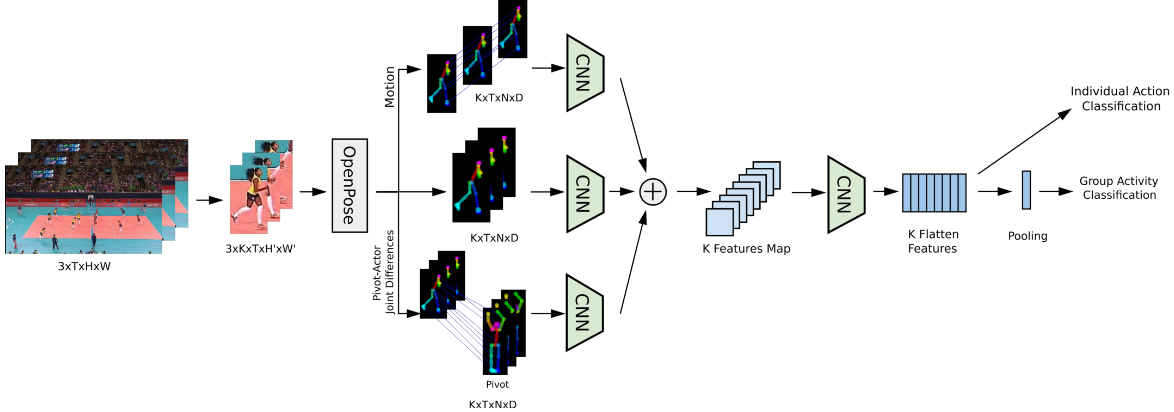
\includegraphics[width=0.9\linewidth]{szkielety.png}
    \caption{Hierarchiczny model oparty na sieciach splotowych oraz cechach szkieletowych}
    \label{fig:szkielety-arch}
\end{figure}

W pracy przetestowane zostały dwa podejścia do treningu modelu: 
\begin{itemize}
    \item Rozłączny trening modelu działającego na pojedynczych osobach oraz klasyfikatora. W tym przypadku wymagana są etykiety akcji poszczególnych osób, autor wypróbował również wygenerowanie własnych etykiet poprzez klastrowanie wyjść z wcześniej wytrenowanego już modelu P3D
    \item Trening całościowy modelu
\end{itemize}
Testy przeprowadzone zostały na zbiorze danych, składającym się z nagrań zagrań w siatkówce \cite{Ibrahim2015}, osiągając najlepszą skuteczność dla całościowego treningu modelu wynoszącą 91\%. 

\subsubsection{Hierarchiczne modelowanie czasowe} 
Ibrahim et al. \cite{Ibrahim2015} zaproponował w swojej pracy hierarchiczny model oparty na sieciach LSTM oraz cechach RGB wyekstrahowanych przy pomocy wcześniej wytrenowanej sieci AlexNet \cite{alexnet}. 

Architektura modelu składa się z dwóch sieci LSTM, połączonych w hierarchię. Zdaniem pierwszej z sieci jest analiza aktywności indywidualnej. Jest ona nakładana na każdą z osób wykrytych w akcji. Sieć składa się z 9 kroków czasowych oraz 3000 stanów ukrytych, na wejściu otrzymuje sekwencje składającą się z cech RGB poszczególnej osoby, na wyjściu zwracane są wszystkie stany ukryte ostatniej warstwy LSTM sieci. Następnie wykonana zostaje transformacja MaxPooling'u stanów ukrytych po osobach, która jest wejściem do kolejnego modelu LSTM składającego się z 9 kroków czasowych oraz 500 stanów ukrytych. Architektura modelu została przedstawiona na rysunku \ref{fig:ibrahim-arch}. 
\begin{figure}[!h]
    \centering 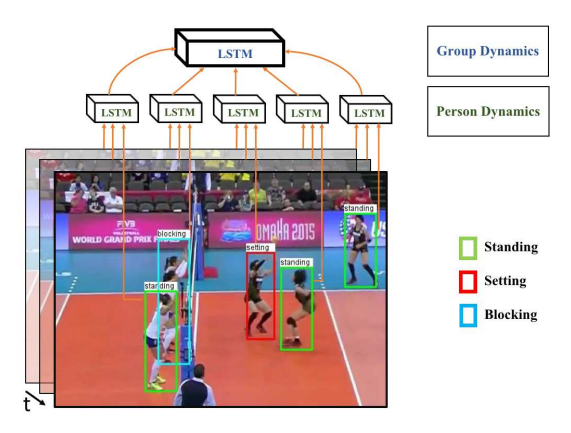
\includegraphics[width=0.9\linewidth]{ibrahim.png}
    \caption{Hierarchiczny model oparty na sieciach LSTM oraz cechach RGB}
    \label{fig:ibrahim-arch}
\end{figure}
Trening modeli został przeprowadzony osobno dla każdej z sieci w hierarchii. Dla modelu niższego stopnia wykorzystane zostały etykiety aktywności indywidualnych. Trening modelu wyższego poziomu odbywa się przy zamrożeniu wag modelu niższego poziomu, wykorzystuje już docelowe etykiety aktywności grupowych. 

Model osiąga skuteczność 81.5\% na zbiorze danych Collective Activity Dataset \cite{collective_ds}, jednak dla bardziej złożonych zbiorach danych radzi sobie gorzej, osiągając skuteczność wynoszącą 51.1\% na zbiorze danych zagrań w siatkówce \cite{Ibrahim2015}.

\subsection{Modele oparte na cechach całego obrazu}
Charakterystyczną cechą tego podejścia jest zaawansowana analiza klatek nagrania. Transformuje ono zagadnienie klasyfikacji aktywności grupowej w ogólny problem klasyfikacji wideo, gdzie liczba osób na nagraniu nie ma znaczenia. Może to być jedna osoba, grupa, tłum, a nawet brak osób. Dzięki temu nie wymaga ono tak intensywnego wstępnego przetworzenia danych i jest bardziej oszczędne obliczeniowo. 

\subsubsection{Dwukierunkowy model LSTM oparty na cecach RGB}
Ullah A. et al. \cite{Ullah2017} w swojej pracy proponuję podejście, które polega na ekstrakcji cech RGB za pomocą sieci splotowych oraz kodowaniu sekwencji za pomocą dwóch wzajemnie połączonych warstw LSTM, która następnie podlega klasyfikacji. Architektura rozwiązania została przedstawiona na rysunku \ref{fig:ullah-arch}
\begin{figure}[!h]
    \centering 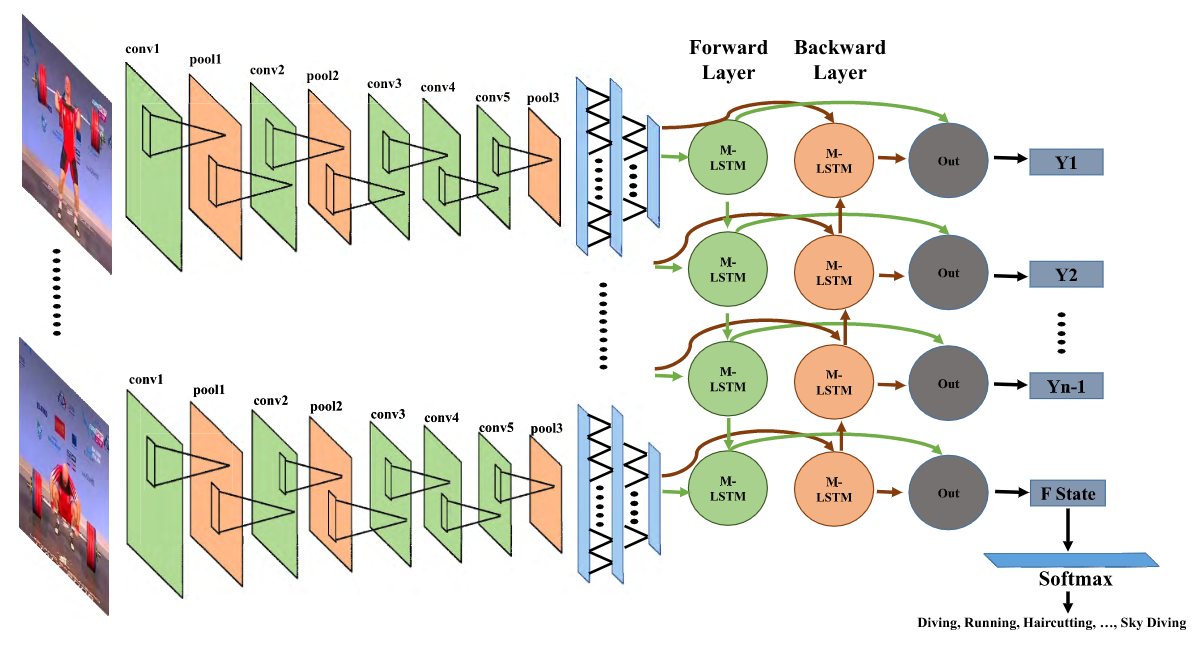
\includegraphics[width=0.9\linewidth]{ullah.png}
    \caption{Dwukierunkowy model LSTM oparty na cechach RGB}
    \label{fig:ullah-arch}
\end{figure}
Model klasyfikuje nagrania sekunda po sekundzie, wybierając z każdej sekundy co 6 klatkę. Został przetestowany na zbiorze danych wideo pochodzących z serwisu YouTube \cite{yt_dataset}, osiągając skuteczność 92.84\%. 

\subsection{Rozwiązania komercyjne}
\subsubsection{AutoML} 
Na rynku dostępne są narzędzia pozwalające na wytworzenie modelu uczenia maszynowego o dowolnym zastosowaniu (m.in. klasyfikacja aktywności), bez konieczności projektowania architektury. Przykładem takiego narzędzia jest AutoML (Automated Machine Learning)\cite{automl} firmy Google. 

Podejście to opiera się na wybraniu zadania jakie ma realizować model (jaki typ danych model otrzyma na wejściu, jaki ma być rezultat modelu np. klasyfikacja). Następnie proces w oparciu o analizowany zbiór danych oraz udostępnione informacje automatycznie wybiera odpowiedni typ modelu uczenia maszynowego, który najlepiej pasuje do określonego problemu. Po wyborze modelu, proces AutoML trenuje go, dopasowując parametry i wagi do danych treningowych, wykonuje automatycznego wyszukania architektury (NAS), dokonuje optymalizacji modelu, wybierając optymalne parametry i techniki regularyzacji. Proces zwraca najlepszy znaleziony model. 

Ze względu, że jest to zastosowanie komercyjne, szczegółowe informacje na temat działania modelu nie są publicznie dostępne.